% Section 2 - Image processing
% Roberto Masocco <roberto.masocco@uniroma2.it>
% June 7, 2023

% ### Image processing ###
\section{Image processing}
\graphicspath{{figs/section2/}}

% --- Vision in robotics ---
\begin{frame}{Vision in robotics}{Sensors characteristics}
	\begin{columns}
		\column{.5\textwidth}
		\textbg{Visual sensors}, commonly referred to as \textbg{cameras}, are sensors that provide \textbg{images} as output, encoded in \textbg{frames}, \emph{i.e.}, \textbg{matrices} of data points. They are usually made of:
		\begin{itemize}
			\item one or more \textbg{optical lenses}, to focus light on the sensor;
			\item a \textbg{sensor}, to convert light into electrical signals;
			\item a \textbg{processing unit}, to convert electrical signals into images, optionally applying \textbg{post-processing} steps.
		\end{itemize}

		\column{.5\textwidth}
		\begin{figure}
			\centering
			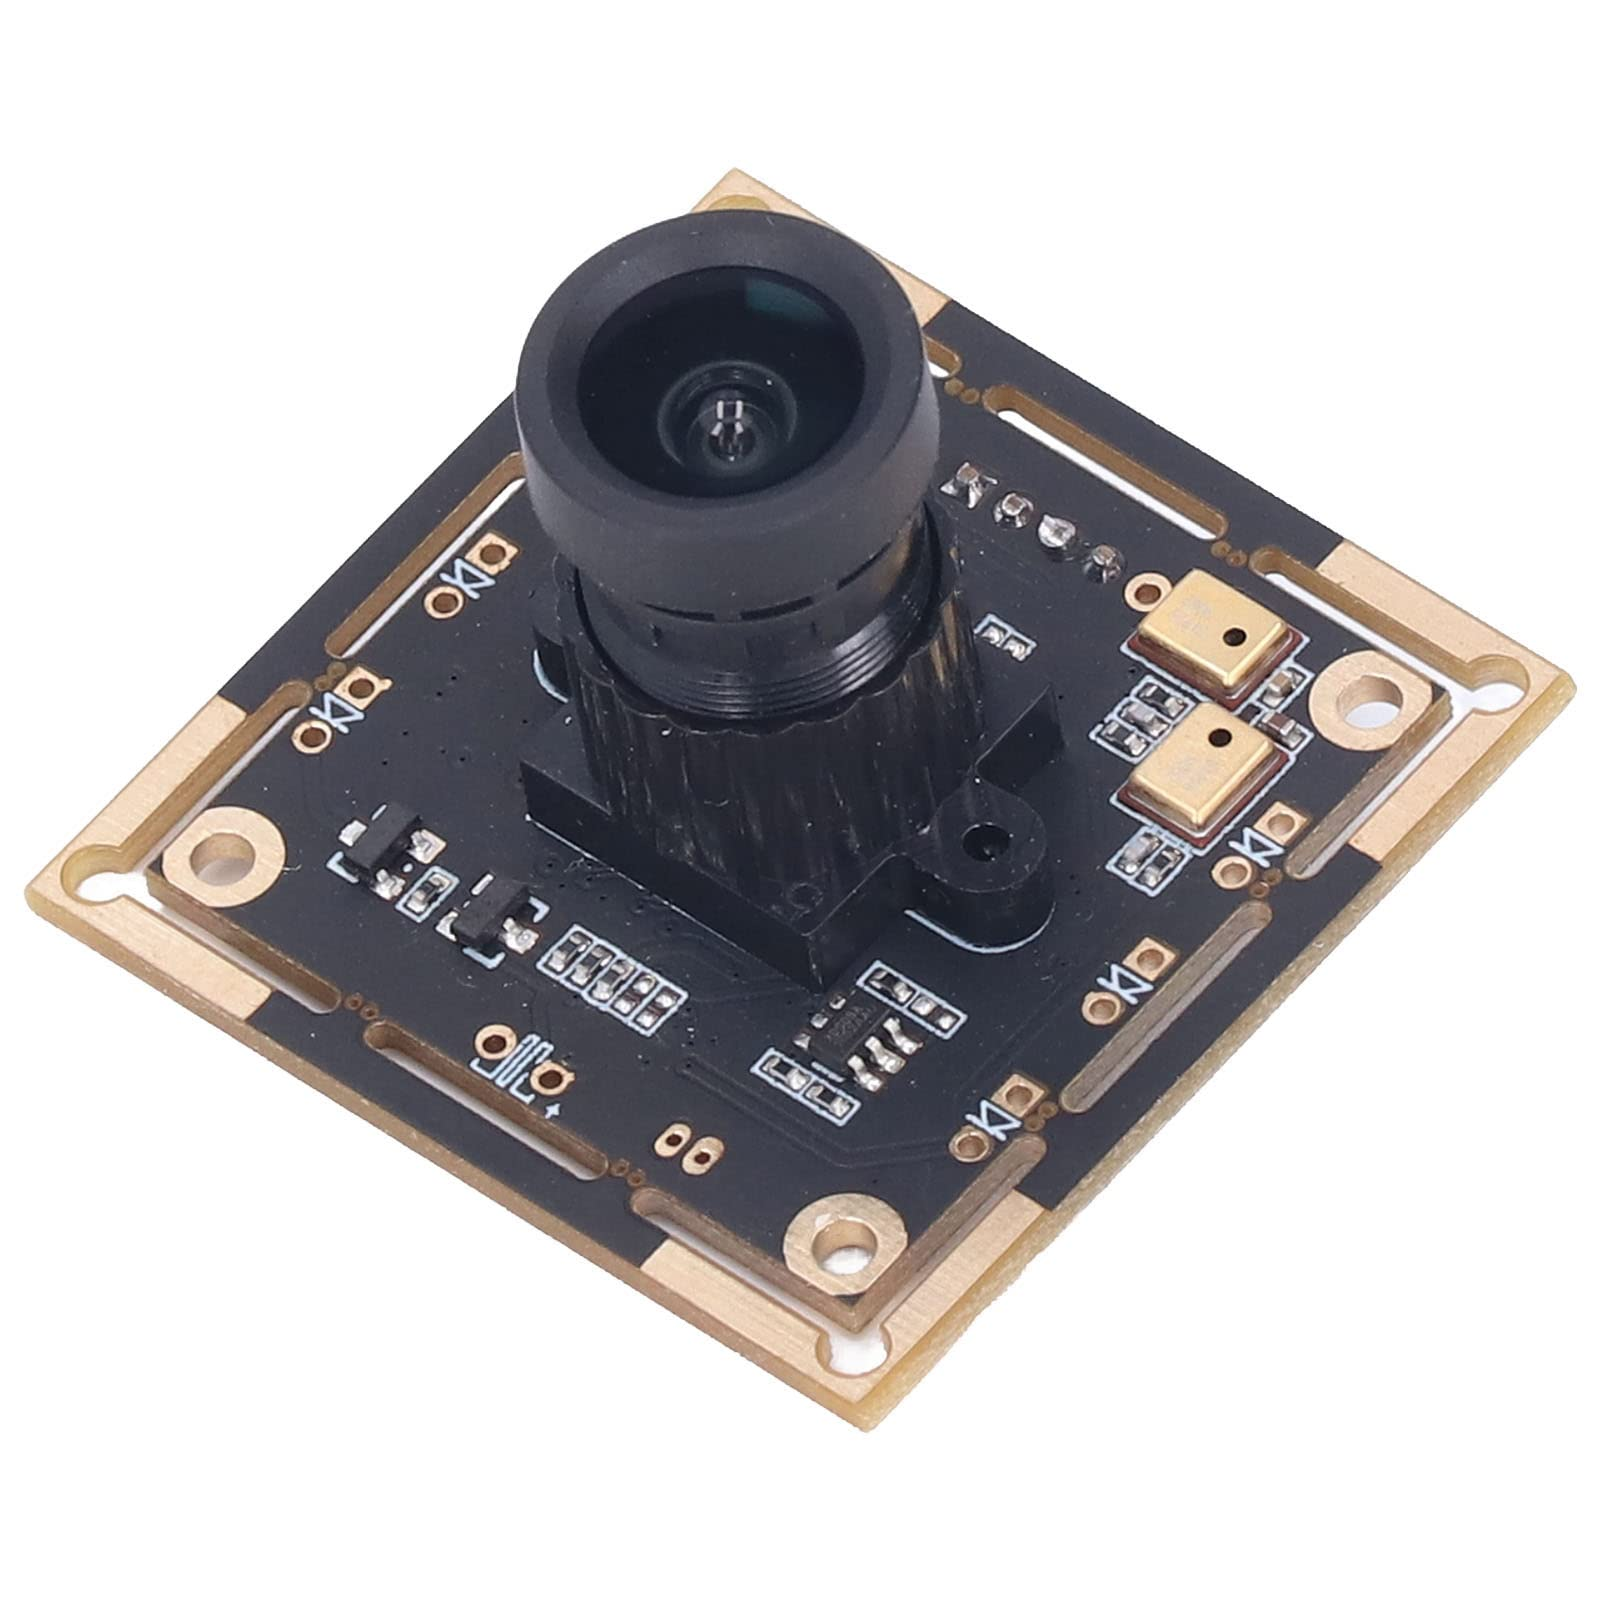
\includegraphics[width=.7\textwidth]{rgbcam}
			\caption{RGB USB camera.}
			\label{fig:rgbcam}
		\end{figure}
	\end{columns}
\end{frame}
\begin{frame}{Vision in robotics}{Sensors characteristics}
	\begin{columns}
		\column{.5\textwidth}
		\begin{block}{}
			\centering
			\textbf{Light might not belong to the visible band of the spectrum.}
		\end{block}

		\column{.5\textwidth}
		\begin{figure}
			\centering
			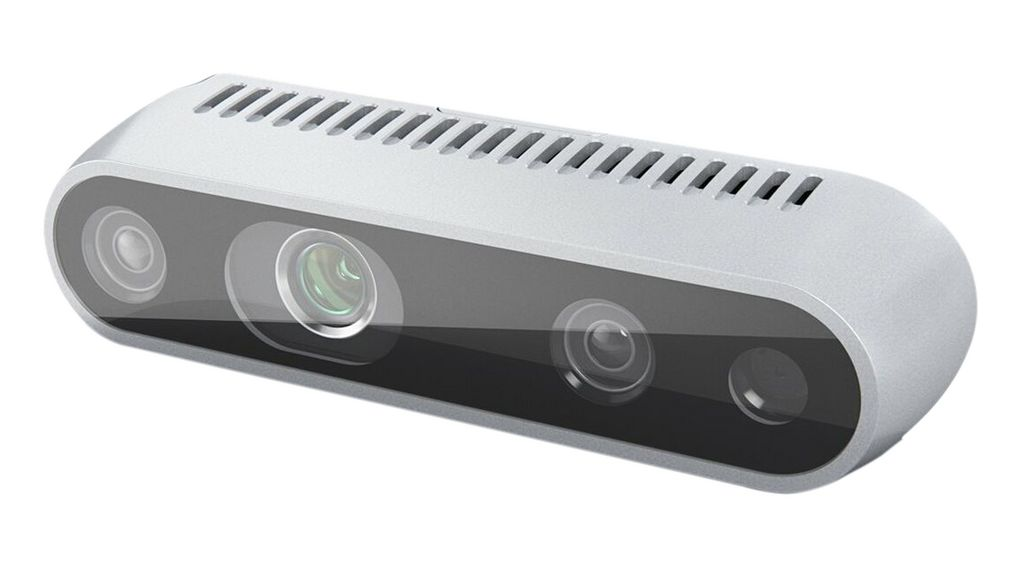
\includegraphics[width=\textwidth]{d435i}
			\caption{Intel RealSense D435i depth camera: RGB and IR sensors.}
			\label{fig:d435i}
		\end{figure}
	\end{columns}
\end{frame}
\begin{frame}{Vision in robotics}{Sensors characteristics}
	\begin{columns}
		\column{.5\textwidth}
		\textbg{Cameras} are usually characterized by:
		\begin{itemize}
			\item \textbg{resolution}, \emph{i.e.}, the number of pixels in the image;
			\item \textbg{field of view}, \emph{i.e.}, the angular extension of the scene (horizontal and vertical);
			\item \textbg{frame rate}, \emph{i.e.}, the number of frames per second;
			\item \textbg{dynamic range}, \emph{i.e.}, the ratio between the maximum and minimum measurable light intensity.
		\end{itemize}

		\column{.5\textwidth}
		\begin{figure}
			\centering
			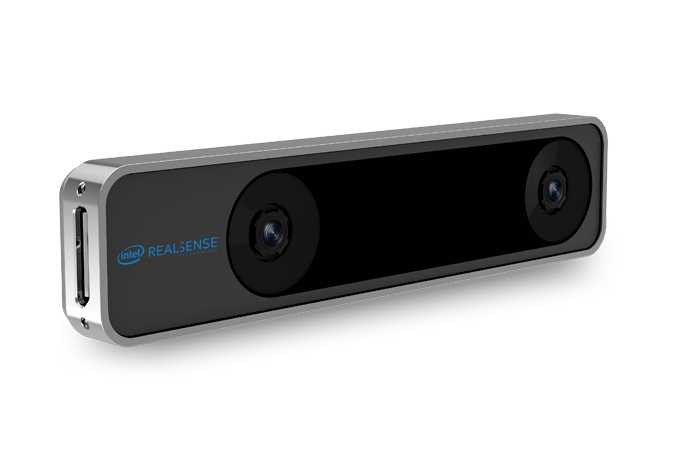
\includegraphics[width=\textwidth]{t265}
			\caption{Intel RealSense T265 tracking camera: two fisheye sensors.}
			\label{fig:t265}
		\end{figure}
	\end{columns}
\end{frame}
\begin{frame}{Vision in robotics}{Sensors characteristics}
	\begin{columns}
		\column{.5\textwidth}
		\begin{block}{}
			\centering
			\textbf{Cameras, and image processing algorithms in general, are usually characterized by a trade-off between resolution and frame rate.}
		\end{block}

		\column{.5\textwidth}
		\begin{figure}
			\centering
			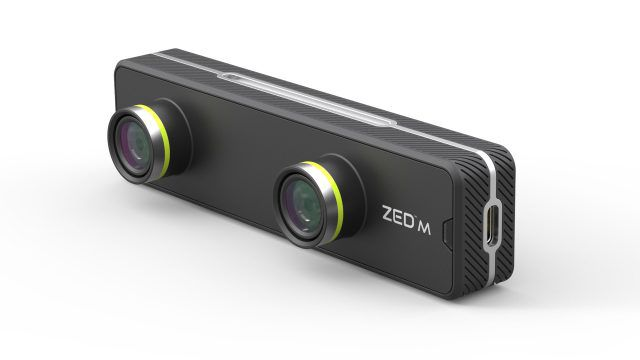
\includegraphics[width=\textwidth]{zedm}
			\caption{ZED Mini stereo tracking camera.}
			\label{fig:zedm}
		\end{figure}
	\end{columns}
\end{frame}
\begin{frame}{Vision in robotics}{Main use cases}
	Visual sensors are usually employed in robotics for:
	\begin{itemize}
		\item \textbg{object detection}, \emph{i.e.}, identifying objects in the scene;
		\item \textbg{object tracking}, \emph{i.e.}, following objects in the scene;
		\item \textbg{localization}, \emph{i.e.}, estimating the robot's position in the environment;
		\item \textbg{mapping}, \emph{i.e.}, building a model of the environment.
	\end{itemize}
	\vspace{.5cm}
	Using the sensor is not enough: \textbg{algorithms} are needed to perform these tasks.\\
	Such algorithms usually run in separate modules.
\end{frame}

% --- Types of frames ---
\begin{frame}{Types of frames}{RGB frame}
	\begin{figure}
		\centering
		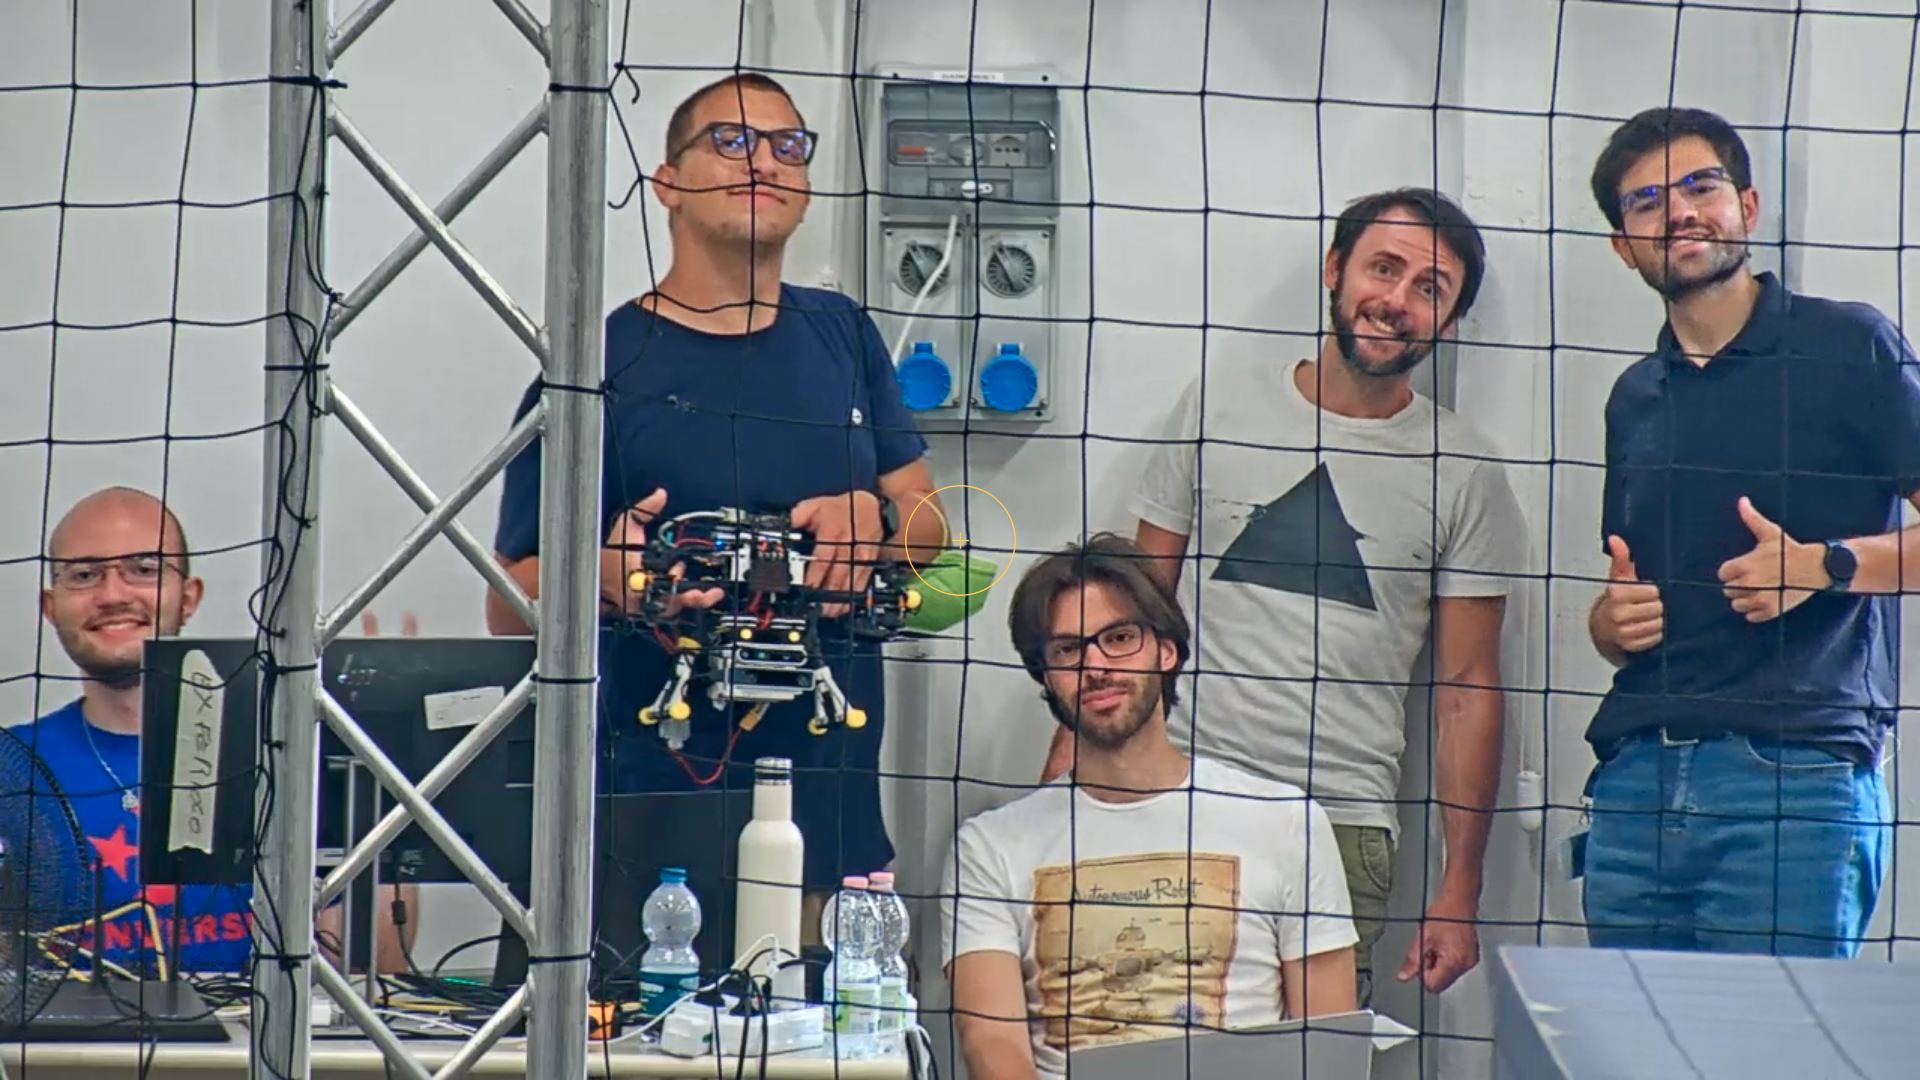
\includegraphics[width=.63\textwidth]{rgb}
		\caption{RGB frame: each pixel contains at least the intensities of the red, green and blue components of the corresponding point in the scene.}
		\label{fig:rgb}
	\end{figure}
\end{frame}
\begin{frame}{Types of frames}{IR frame}
	\begin{figure}
		\centering
		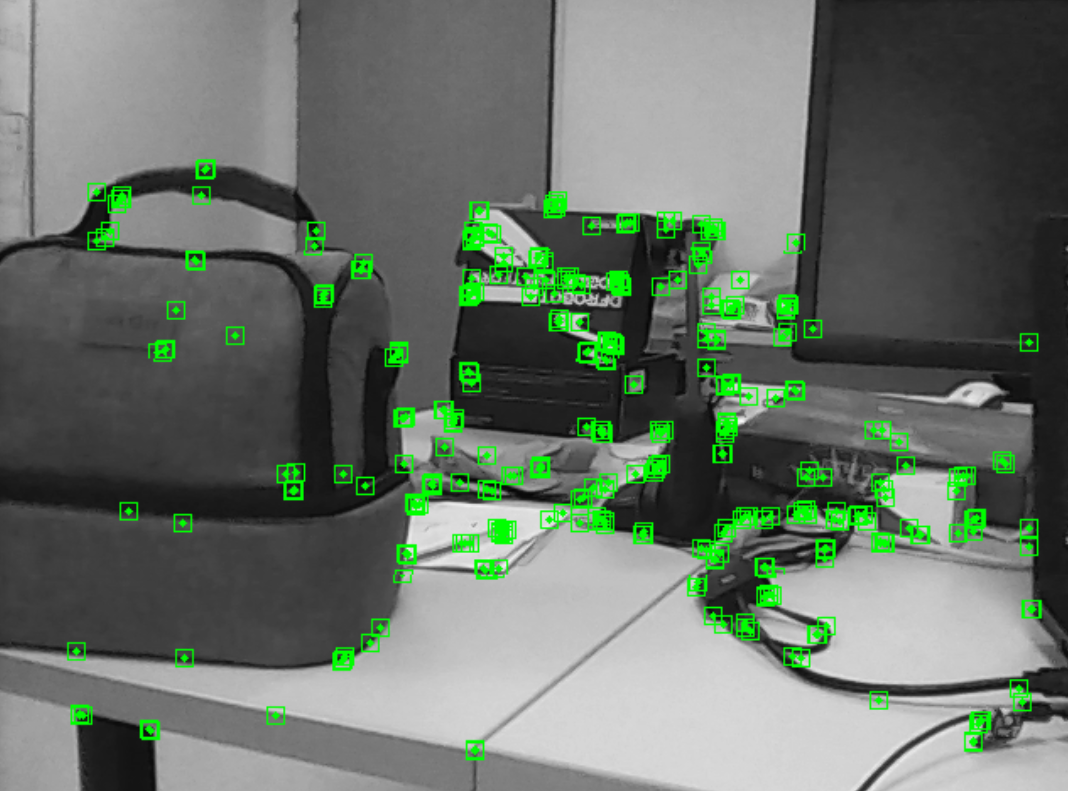
\includegraphics[width=.5\textwidth]{ir}
		\caption{IR frame: each pixel contains the intensity of the corresponding point in the scene.}
		\label{fig:ir}
	\end{figure}
\end{frame}
\begin{frame}{Types of frames}{Depth map frame}
	\begin{figure}
		\centering
		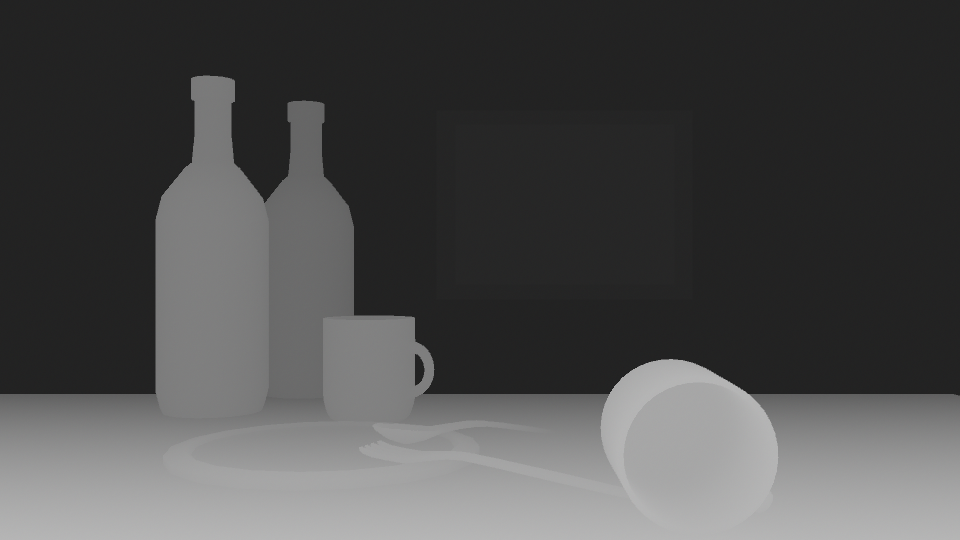
\includegraphics[width=.68\textwidth]{depthmap}
		\caption{Depth map frame: each pixel contains the distance of the corresponding point from the camera.}
		\label{fig:depthmap}
	\end{figure}
\end{frame}

% --- Lens distorsion ---
\begin{frame}{Lens distorsion}{Camera calibration and rectification}
	\begin{columns}
		\column{.5\textwidth}
		\textbg{Pinhole cameras} generally introduce \textbg{radial distorsion} in the images they produce, \emph{i.e.}, \textbg{straight lines appear curved}. This is due to how the light enters the camera through the lens.
		\newline\newline
		A \textbg{camera calibration} procedure is needed to estimate the parameters of the \textbg{distorsion model}, so that a \textbg{rectification map} can then be applied to each frame.

		\column{.5\textwidth}
		\begin{figure}
			\centering
			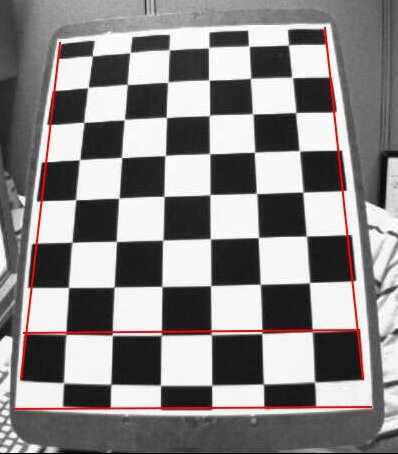
\includegraphics[width=.6\textwidth]{radial}
			\caption{Checkerboard pattern used for camera calibration in the presence of radial distortion.}
			\label{fig:radial}
		\end{figure}
	\end{columns}
\end{frame}
\begin{frame}{Lens distorsion}{Camera calibration and rectification}
	\begin{columns}
		\column{.5\textwidth}
		The calibration procedure usually involves moving a \textbg{checkerboard} of known dimensions in front of the camera, and taking several pictures of it from different angles.
		\newline\newline
		An \textbg{estimation model} can then be used to estimate the parameters of the distorsion model, which can then be used to build the rectification map.

		\column{.5\textwidth}
		\begin{figure}
			\centering
			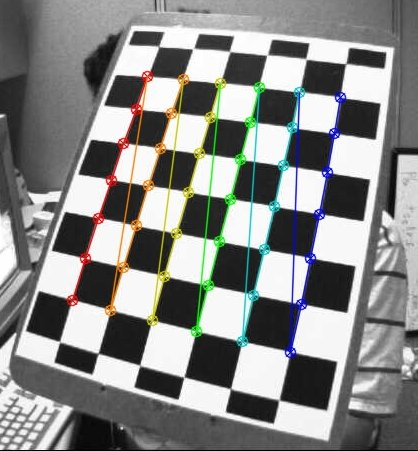
\includegraphics[width=.6\textwidth]{calibration}
			\caption{A frame from a checkerboard calibration procedure.}
			\label{fig:calibration}
		\end{figure}
	\end{columns}
\end{frame}
\begin{frame}{Lens distorsion}{Camera calibration and rectification}
	\begin{columns}
		\column{.5\textwidth}
		The \textbg{rectification map} is a \textbg{lookup table} that associates each pixel in the original frame with a pixel in the rectified frame, \textbg{interpolating} when necessary.
    \newline\newline
    It is usually stored in \textbg{configuration files}, and must be applied to each frame before it can be used by other algorithms.
    \vspace{.45cm}
    \begin{block}{}
      \centering
      \textbf{ROS 2 offers the \href{https://navigation.ros.org/tutorials/docs/camera_calibration.html}{\color{blue}\underline{\texttt{cameracalibrator}}} tool in the \texttt{camera\_calibration} package to perform camera calibration.}
    \end{block}

		\column{.5\textwidth}
		\begin{figure}
			\centering
			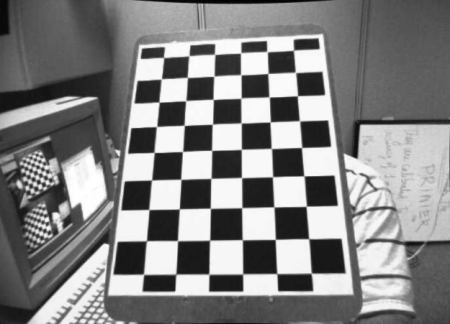
\includegraphics[width=.9\textwidth]{calibrated}
			\caption{Checkerboard pattern after rectification.}
			\label{fig:calibrated}
		\end{figure}
	\end{columns}
\end{frame}
